\chapter {Odpowiedzi skokowe}

\section{Wykresy odpowiedzi skokowych}

W celu zbadania charakterystyki zakłóceń, dokonano ich skoku z punktu pracy (Z=0) odpowiednio o +10, +20 i -10. Wyniki eksperymentu przedstawiono na rysunku \ref{odp_skok}:

\begin{figure}[h!]

	\centering
	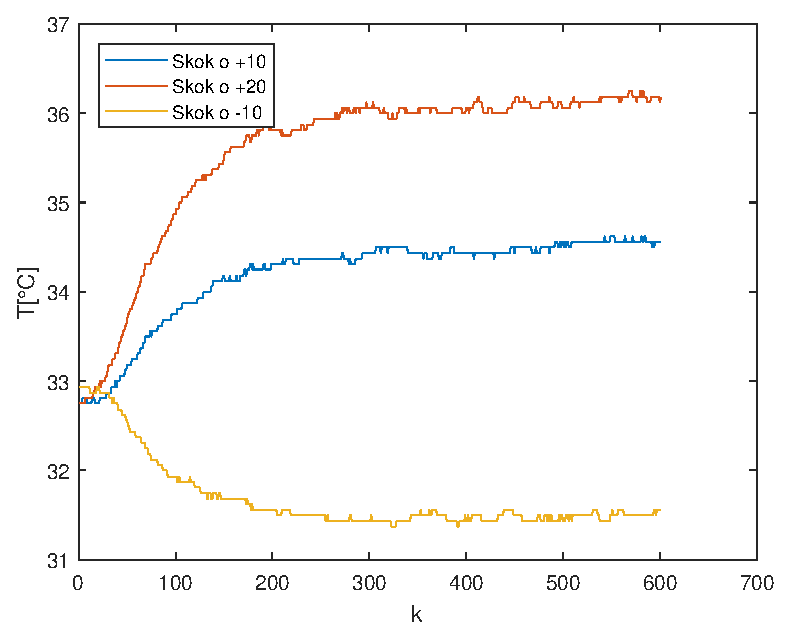
\includegraphics[scale=1]{Rys/LAB2_StepResponses_Z2.eps}
	\caption{Odpowiedzi skokowe toru zakłócenie-wyjście}
	\label{odp_skok}

\end{figure}


\section{Wzmocnienie statyczne}
\label{zad2_wzmocnienie}
Wzmocnienie statyczne, czyli stosunek pomiędzy zmianą wartości wyjścia na zmianę wartości (skok) sterowania lub zakłóceń, tzn:
\begin{equation}
K_{\mathrm{stat}} = \frac{\Delta Y}{\Delta Z}
\label{zad2_wzm_statyczne_wzor}
\end{equation}

Dla skoku o 10, wzmocnienie jest równe:
\begin{equation}
K_{\mathrm{stat}}\approx \frac{34,56-32,75}{10}=0,181
\label{zad2_wzm_statyczne_wzor1}
\end{equation}




Dla skoku o 20, wzmocnienie jest równe:
\begin{equation}
K_{\mathrm{stat}}\approx \frac{36,12-32,75}{-10}=0,1685
\label{zad2_wzm_statyczne_wzor2}
\end{equation}

Dla skoku o -10, wzmocnienie jest równe:
\begin{equation}
K_{\mathrm{stat}}\approx \frac{31,5-32,93}{10}=0,143
\label{zad2_wzm_statyczne_wzor3}
\end{equation}



Występuje pewna rozbieżność w wyliczonych wartościach, jednak nie jest ona ogromna, można uznać obiekt za względnie liniowy o wzmocnieniu statycznym równym przykładowo wzmocnieniu wyliczonym przy największym skoku tj. \num {0,1685}.


%ś

